\documentclass[9.2pt,twocolumn]{article}
\usepackage{lmodern}
\usepackage{amssymb,amsmath}
\usepackage{ifxetex,ifluatex}
\usepackage{fixltx2e} % provides \textsubscript
\ifnum 0\ifxetex 1\fi\ifluatex 1\fi=0 % if pdftex
  \usepackage[T1]{fontenc}
  \usepackage[utf8]{inputenc}
\else % if luatex or xelatex
  \ifxetex
    \usepackage{mathspec}
  \else
    \usepackage{fontspec}
  \fi
  \defaultfontfeatures{Ligatures=TeX,Scale=MatchLowercase}
\fi
% use upquote if available, for straight quotes in verbatim environments
\IfFileExists{upquote.sty}{\usepackage{upquote}}{}
% use microtype if available
\IfFileExists{microtype.sty}{%
\usepackage{microtype}
\UseMicrotypeSet[protrusion]{basicmath} % disable protrusion for tt fonts
}{}
\usepackage[left=1.5cm,right=1.5cm,top=2.2cm,bottom=2cm]{geometry}
\usepackage{hyperref}
\PassOptionsToPackage{usenames,dvipsnames}{color} % color is loaded by hyperref
\hypersetup{unicode=true,
            pdftitle={Ethiopia},
            pdfauthor={Commitment to Human Capital - Scorecard},
            colorlinks=true,
            linkcolor=Maroon,
            citecolor=Blue,
            urlcolor=blue,
            breaklinks=true}
\urlstyle{same}  % don't use monospace font for urls
\usepackage{graphicx,grffile}
\makeatletter
\def\maxwidth{\ifdim\Gin@nat@width>\linewidth\linewidth\else\Gin@nat@width\fi}
\def\maxheight{\ifdim\Gin@nat@height>\textheight\textheight\else\Gin@nat@height\fi}
\makeatother
% Scale images if necessary, so that they will not overflow the page
% margins by default, and it is still possible to overwrite the defaults
% using explicit options in \includegraphics[width, height, ...]{}
\setkeys{Gin}{width=\maxwidth,height=\maxheight,keepaspectratio}
\IfFileExists{parskip.sty}{%
\usepackage{parskip}
}{% else
\setlength{\parindent}{0pt}
\setlength{\parskip}{6pt plus 2pt minus 1pt}
}
\setlength{\emergencystretch}{3em}  % prevent overfull lines
\providecommand{\tightlist}{%
  \setlength{\itemsep}{0pt}\setlength{\parskip}{0pt}}
\setcounter{secnumdepth}{0}
% Redefines (sub)paragraphs to behave more like sections
\ifx\paragraph\undefined\else
\let\oldparagraph\paragraph
\renewcommand{\paragraph}[1]{\oldparagraph{#1}\mbox{}}
\fi
\ifx\subparagraph\undefined\else
\let\oldsubparagraph\subparagraph
\renewcommand{\subparagraph}[1]{\oldsubparagraph{#1}\mbox{}}
\fi

%%% Use protect on footnotes to avoid problems with footnotes in titles
\let\rmarkdownfootnote\footnote%
\def\footnote{\protect\rmarkdownfootnote}

%%% Change title format to be more compact
\usepackage{titling}

% Create subtitle command for use in maketitle
\providecommand{\subtitle}[1]{
  \posttitle{
    \begin{center}\large#1\end{center}
    }
}

\setlength{\droptitle}{-2em}

  \title{Ethiopia}
    \pretitle{\vspace{\droptitle}\centering\huge}
  \posttitle{\par}
    \author{Commitment to Human Capital - Scorecard}
    \preauthor{\centering\large\emph}
  \postauthor{\par}
    \date{}
    \predate{}\postdate{}
  
\usepackage{fancyhdr}

\pagestyle{fancy}

\usepackage[table]{xcolor} \usepackage{xcolor} \usepackage{graphicx} \usepackage{eurosym} \usepackage{booktabs,xcolor}

\rhead{Africa Human Capital Project - \today}
\rfoot[C]{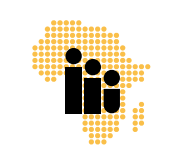
\includegraphics[width=2cm]{static/footer3.png}}
\fancypagestyle{plain}{\pagestyle{fancy}} \pagenumbering{gobble}

\usepackage{pagecolor}

\pagecolor{white}

\usepackage{fourier} \usepackage[fontsize=8.7pt]{scrextend} \usepackage{float} \usepackage[utf8]{inputenc} \usepackage{caption}

\captionsetup[table]{position=bottom}

\begin{document}
\maketitle

\definecolor{bondiblue}{rgb}{0.0, 0.58, 0.71}
\newcommand\boldblue[1]{\textcolor{bondiblue}{\textbf{#1}}}

This scorecard presents a snapshot of the country's commitment to the
human capital agenda and the World Bank Group's support for the social
sectors.

\hypertarget{section}{%
\subsubsection{\texorpdfstring{\textcolor{bondiblue}{\textbf{I\small{NDICATORS IN THE AFRICA HUMAN CAPITAL PLAN}}}}{}}\label{section}}

\begin{itemize}
\item
  \textbf{Human Capital Index.} In Ethiopia the productivity as a future
  worker of a child born today is \textbf{38 percent} as much as it
  could be. The HCI has three components: survival to age 5, health, and
  education. For more information on human capital outcomes and the HCI,
  please see the country two-pager on
  \textcolor{bondiblue}{\textbf{www.worldbank.org/humancapitalproject}}
\item
  \textbf{Adolescent Fertility Rate.} In Ethiopia, there are \textbf{62
  births} per 1,000 women ages 15-19. This is lower than the Africa
  Human Capital Target for 2023 (83).
\item
  \textbf{Social Protection Coverage.} In Ethiopia, \textbf{13 percent}
  of the poorest quintile is covered by social safety nets. This is
  lower than the Africa Human Capital Target for 2023 (30).
\item
  \textbf{Open Defecation.} In Ethiopia, \textbf{27 percent} of the
  population practices open defecation. This is higher than the Africa
  Human Capital Target for 2023 (15).
\end{itemize}

\hypertarget{section-1}{%
\subsubsection{\texorpdfstring{\textcolor{bondiblue}{\textbf{I\small{NDICATORS ON WOMEN'S EMPOWERMENT}}}}{}}\label{section-1}}

\begin{itemize}
\item
  \textbf{Total Fertility Rate.} In Ethiopia, the total fertility rate
  is \textbf{4.1} births per woman. This is lower than both the average
  for its region (4.5) and the average for its income group (4.7).
\item
  \textbf{Contraceptive Prevalence.} In Ethiopia, \textbf{37 percent} of
  women ages 15-49 uses some form of contraceptive method. This is
  higher than both the average for its region (31) and the average for
  its income group (28).
\item
  \textbf{Women, Business and the Law Index.} This index measures gender
  equality in the law (how the economic decisions women make are
  affected by the law), with a larger value showing higher gender
  equality. In Ethiopia, the value is \textbf{72} out of 100. This is
  higher than both the average for its region (70) and the average for
  its income group (68).
\item
  \textbf{Net Enrolment Rate in Secondary School.} In Ethiopia,
  \textbf{30 percent} of girls of secondary-school age are enrolled in
  secondary school. This is lower than the average for its region (35)
  but higher than the average for its income group (29).
\end{itemize}

\hypertarget{section-2}{%
\subsubsection{\texorpdfstring{\textcolor{bondiblue}{\textbf{D\small{OMESTIC RESOURCE USE AND MOBILIZATION}}}}{}}\label{section-2}}

\begin{itemize}
\item
  \textbf{Health Spending.} Ethiopia spends \textbf{6 percent} of its
  government budget on health. This is lower than both the regional
  average (7.6) and the average for its income group (6.8).
\item
  \textbf{Education Spending.} Ethiopia spends \textbf{27.1 percent} of
  its government budget on education. This is higher than both the
  regional average (15.3) and the average for its income group (15.5).
\item
  \textbf{Social Protection Spending.} Ethiopia spends \textbf{10.8
  percent} of its government budget on social protection. This is higher
  than both the regional average (9.9) and the average for its income
  group (10.8).
\end{itemize}

\begin{flushright}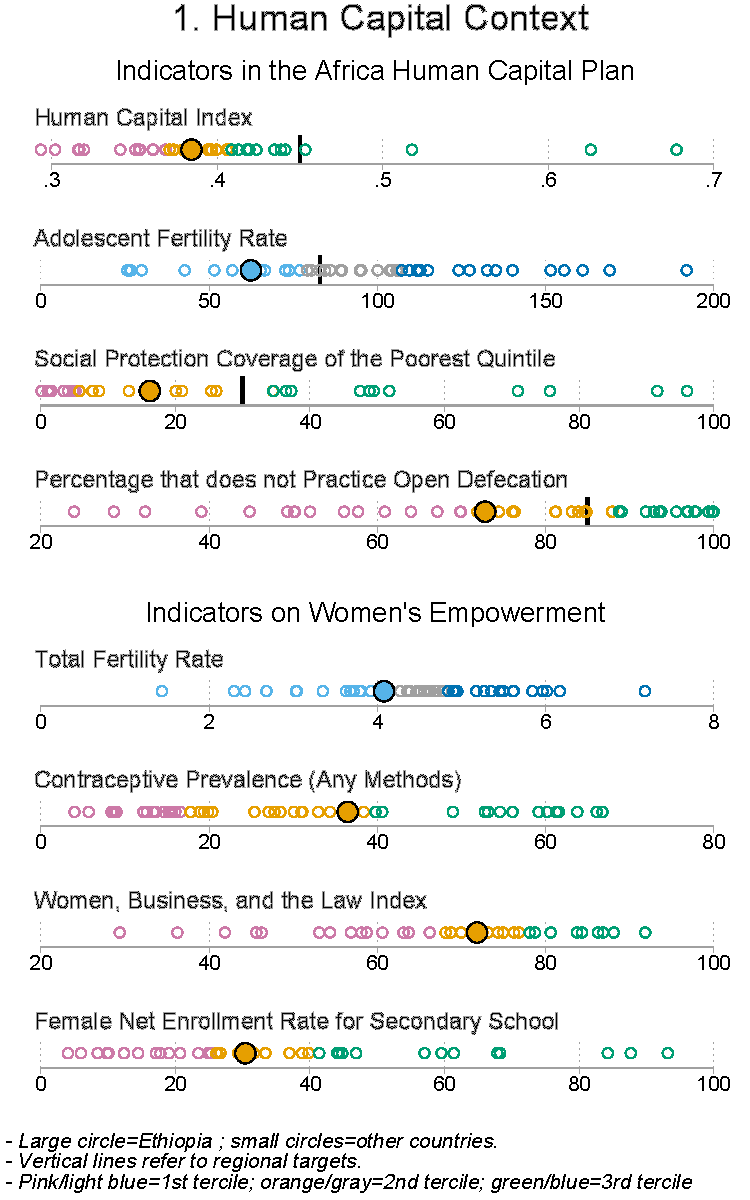
\includegraphics[width=1\linewidth]{charts/all_mf_ETH} \end{flushright}

\begin{flushright}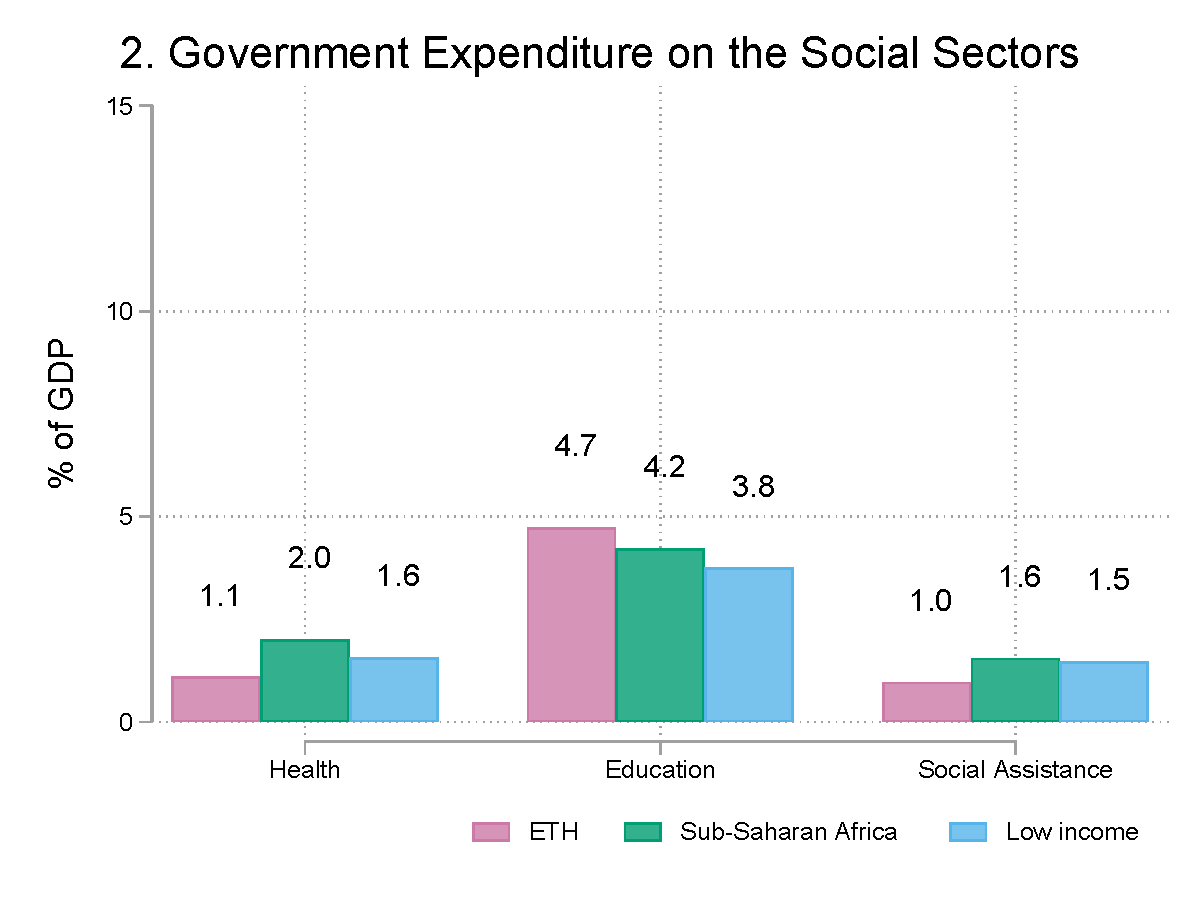
\includegraphics[width=1\linewidth,height=1.2\textheight]{charts/socsec_ETH} \end{flushright}
\vspace{3mm}

\begin{itemize}
\tightlist
\item
  \textbf{Efficiency of Spending.} The HCI in Ethiopia is \textbf{lower}
  than what would be predicted for its level of per capita government
  spending on the social sectors.
\end{itemize}

\begin{center}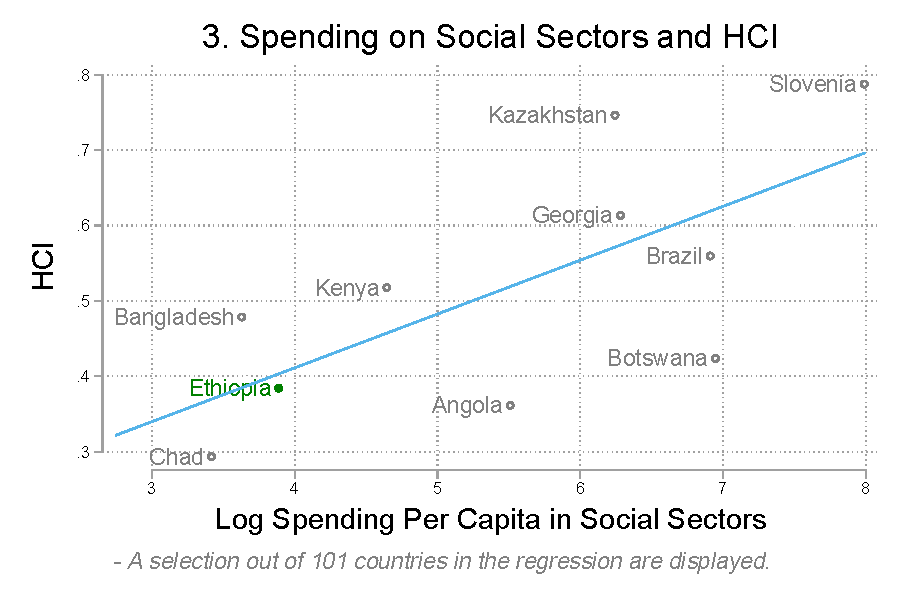
\includegraphics[width=1\linewidth,height=0.5\textheight]{charts/efficiency_ETH} \end{center}

\begin{itemize}
\tightlist
\item
  \textbf{Domestic Resource Mobilization.} The tax revenue in Ethiopia
  is \textbf{7.7} percent of GDP. This is lower than both the regional
  average (16.1) and the average for its income group (14.3).
\end{itemize}

\begin{flushright}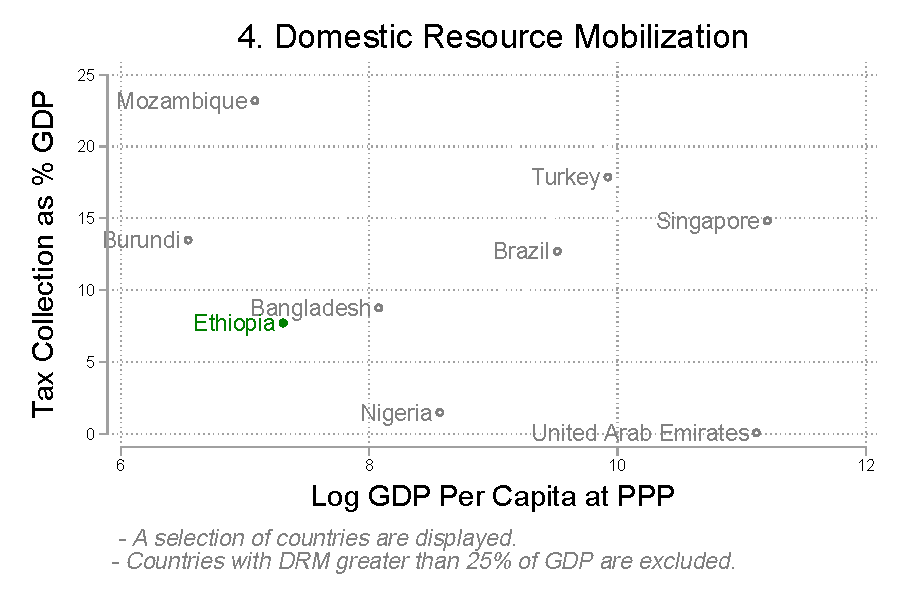
\includegraphics[width=1\linewidth,height=0.5\textheight]{charts/drm_ETH} \end{flushright}

\hypertarget{section-3}{%
\subsubsection{\texorpdfstring{\textcolor{bondiblue}{\textbf{O\small{THER RELEVANT INDICATORS }}}}{}}\label{section-3}}

\begin{itemize}
\item
  \textbf{Human Capital Project.} Ethiopia is part of a network of
  countries committed to the Human Capital agenda.
\item
  \textbf{Building Human Capital.} The Country Policy and Institutional
  Assesment rating for building human resources in Ethiopia is
  \textbf{4.5} (1 is low and 6 is high). This is higher than both the
  regional average (3.5) and the average for its income group (3.5).
  This indicator assesses the national policies and public and private
  sector service delivery that affect access to and quality of health
  and education services.
\item
  \textbf{Identification.} In Ethiopia, \textbf{64.5 percent} of the
  population does not have proof of identity. This is higher than both
  the regional average (33.8) and the average for its income group
  (34.6).
\item
  \textbf{Statistical Data on Human Capital.} In Ethiopia, the latest
  available data point on stunting rate is from 2016. Similarly, the
  latest available data point on Harmonized Learning Outcomes is from
  2010.
\end{itemize}

\hypertarget{section-4}{%
\subsubsection{\texorpdfstring{\textcolor{bondiblue}{\textbf{H\small{OW IS THE WORLD BANK SUPPORTING THE EFFORT?}}}}{}}\label{section-4}}

The following table summarizes the World Bank's investments in Human
Development for Ethiopia, including measures of volume, performance, and
other relevant indicators.

\definecolor{asparagus}{RGB}{3, 158, 115}
\definecolor{blush}{RGB}{204 121 167}
\definecolor{arylideyellow}{RGB}{230 159 0}
\definecolor{blue(ncs)}{rgb}{0.0, 0.53, 0.74}
\definecolor{ashgrey}{rgb}{0.7, 0.75, 0.71}
\definecolor{bleudefrance}{rgb}{0.19, 0.55, 0.91}
\definecolor{iceberg}{rgb}{0.44, 0.65, 0.82}
\begin{table}[H]
\small
\begin{tabular}{lcccc}
\textbf{World Bank Investments in HD} & \textbf{} & \textbf{} & \textbf{} & \textbf{} \\ \hline
\textbf{Indicator} & \textbf{HD} & \textbf{Edu} & \textbf{HNP} & \textbf{SPJ} \\ \hline
\cellcolor{iceberg}HD Portfolio & \cellcolor{iceberg} & \cellcolor{iceberg} & \cellcolor{iceberg} & \cellcolor{iceberg} \\ \hline
USD (million) & 3,688 & 430 & 250 & 3,008 \\ 
\textbf{\% of total} & \cellcolor{asparagus} 32 & \cellcolor{arylideyellow} 4 & \cellcolor{arylideyellow} 2 & \cellcolor{asparagus} 26 \\ 
Diff. from regional average \% & +8 & -3 & -7 & +18 \\ 
Diff. from income group avg \% & +2 & -5 & -10 & +17 \\ \hline
\cellcolor{iceberg}HD FY 20 Lending Program & \cellcolor{iceberg} & \cellcolor{iceberg} & \cellcolor{iceberg} & \cellcolor{iceberg} \\ \hline 
USD (million) & 560 & 60 & 0 & 500 \\ 
\textbf{\% of total} & \cellcolor{asparagus} 100 & \cellcolor{asparagus} 11 & \cellcolor{blush} 0 & \cellcolor{asparagus} 89 \\ 
Diff. from regional average \% & +62 & -0 & -12 & +74 \\ 
Diff. from income group avg \% & +63 & +8 & -15 & +71 \\ \hline
\cellcolor{iceberg}HD Performance & \cellcolor{iceberg} & \cellcolor{iceberg} & \cellcolor{iceberg} & \cellcolor{iceberg} \\ \hline
\textbf{Average Development Outcome} & \cellcolor{arylideyellow} 4 & \cellcolor{blush} 4 & \cellcolor{blush} 4 & \cellcolor{arylideyellow} 4 \\ 
Diff. from regional average \% & -0.24 & -0.30 & -0.54 & -0.16 \\ 
Diff. from income group avg \% & -0.25 & -0.33 & -0.56 & -0.09 \\ 
\% Satisfactory DO & 100 & 100 & 100 & 100 \\  \hline
\textbf{Average Implementation Progress} & \cellcolor{blush} 4 & \cellcolor{blush} 4 & \cellcolor{blush} 4 & \cellcolor{blush} 4 \\ 
Diff. from regional average \% & -0.33 & -0.21 & -0.35 & -0.53 \\ 
Diff. from income group avg \% & -0.31 & -0.22 & -0.38 & -0.39 \\ 
\% Satisfactory IP & 100 & 100 & 100 & 100 \\  \hline
\textbf{Disbursement ratio} & \cellcolor{blush} 0 & \cellcolor{blush} 0 & . & \cellcolor{blush} 0 \\ 
Diff. from regional average \% & -6 & -5 & . & -8 \\ 
Diff. from income group avg \% & -6 & -5 & . & -7 \\ \hline
\cellcolor{iceberg}Other indicators & \cellcolor{iceberg} & \cellcolor{iceberg} & \cellcolor{iceberg} & \cellcolor{iceberg} \\ \hline
\textbf{Average project size (USD mill.)} & \cellcolor{asparagus} 527 & \cellcolor{asparagus} 215 & \cellcolor{asparagus} 250 & \cellcolor{asparagus} 752 \\ 
Diff. from regional average \% & +437 & +145 & +180 & +649 \\ 
Diff. from income group avg \% & +438 & +149 & +176 & +655 \\  \hline
\textbf{\% of portfolio that is co-TTL'd} & \cellcolor{asparagus} 60 & \cellcolor{blush} 0 & \cellcolor{blush} 0 & \cellcolor{asparagus} 73 \\ 
Diff. from regional average \% & +32 & -19 & -28 & +41 \\ 
Diff. from income group avg \% & +30 & -26 & -33 & +38 \\ \hline
\end{tabular}
\caption*{Note: a) \colorbox{blush}{Pink} indicates that the value is within the first tercile of the distribution for all the countries. \colorbox{arylideyellow}{Orange} indicates that the value is within the second tercile. \colorbox{asparagus}{Green} indicates that it is within the third tercile. b) FY20 lending program includes only projects rated A and B. c) DO and IP are on a scale of 1 to 6 where 1 is Highly Unsatisfactory and 6 is Highly Satisfactory. d) Data as of September 5, 2019.}
\end{table}

\begin{itemize}
\item
  \textbf{Human Capital Policy Operations.} Currently, the pipeline for
  Ethiopia does not include any Development Policy Operation with a
  Human Capital-related component or prior action.
\item
  \textbf{Women's Empowerment Project.} Currently, the pipeline for
  Ethiopia does not have an active project focused on women empowerment
  or on sexual and reproductive health.
\end{itemize}

\vspace{-3mm}

\noindent

\rule{9cm}{0.4pt}

This scorecard is intended to be a conversation starter on where a
country is on various aspects of human capital development and the state
of the World Bank's support in the social sectors. The list of
indicators presented here is not exhaustive and should be complemented
with more context specific variables. Most of the indicators are related
to the Africa Human Capital Plan. ~

The sources of data for the different indicators include: the Human
Capital Project, the World Development Indicators, and the World Bank's
internal system to monitor investments. ~

For more information, please contact the Africa Human Capital Project
team:
\href{mailto:AFR_HCP_Team@worldbankgroup.org}{\nolinkurl{AFR\_HCP\_Team@worldbankgroup.org}}


\end{document}
